\begin{figure*}[!t]
  \centering
  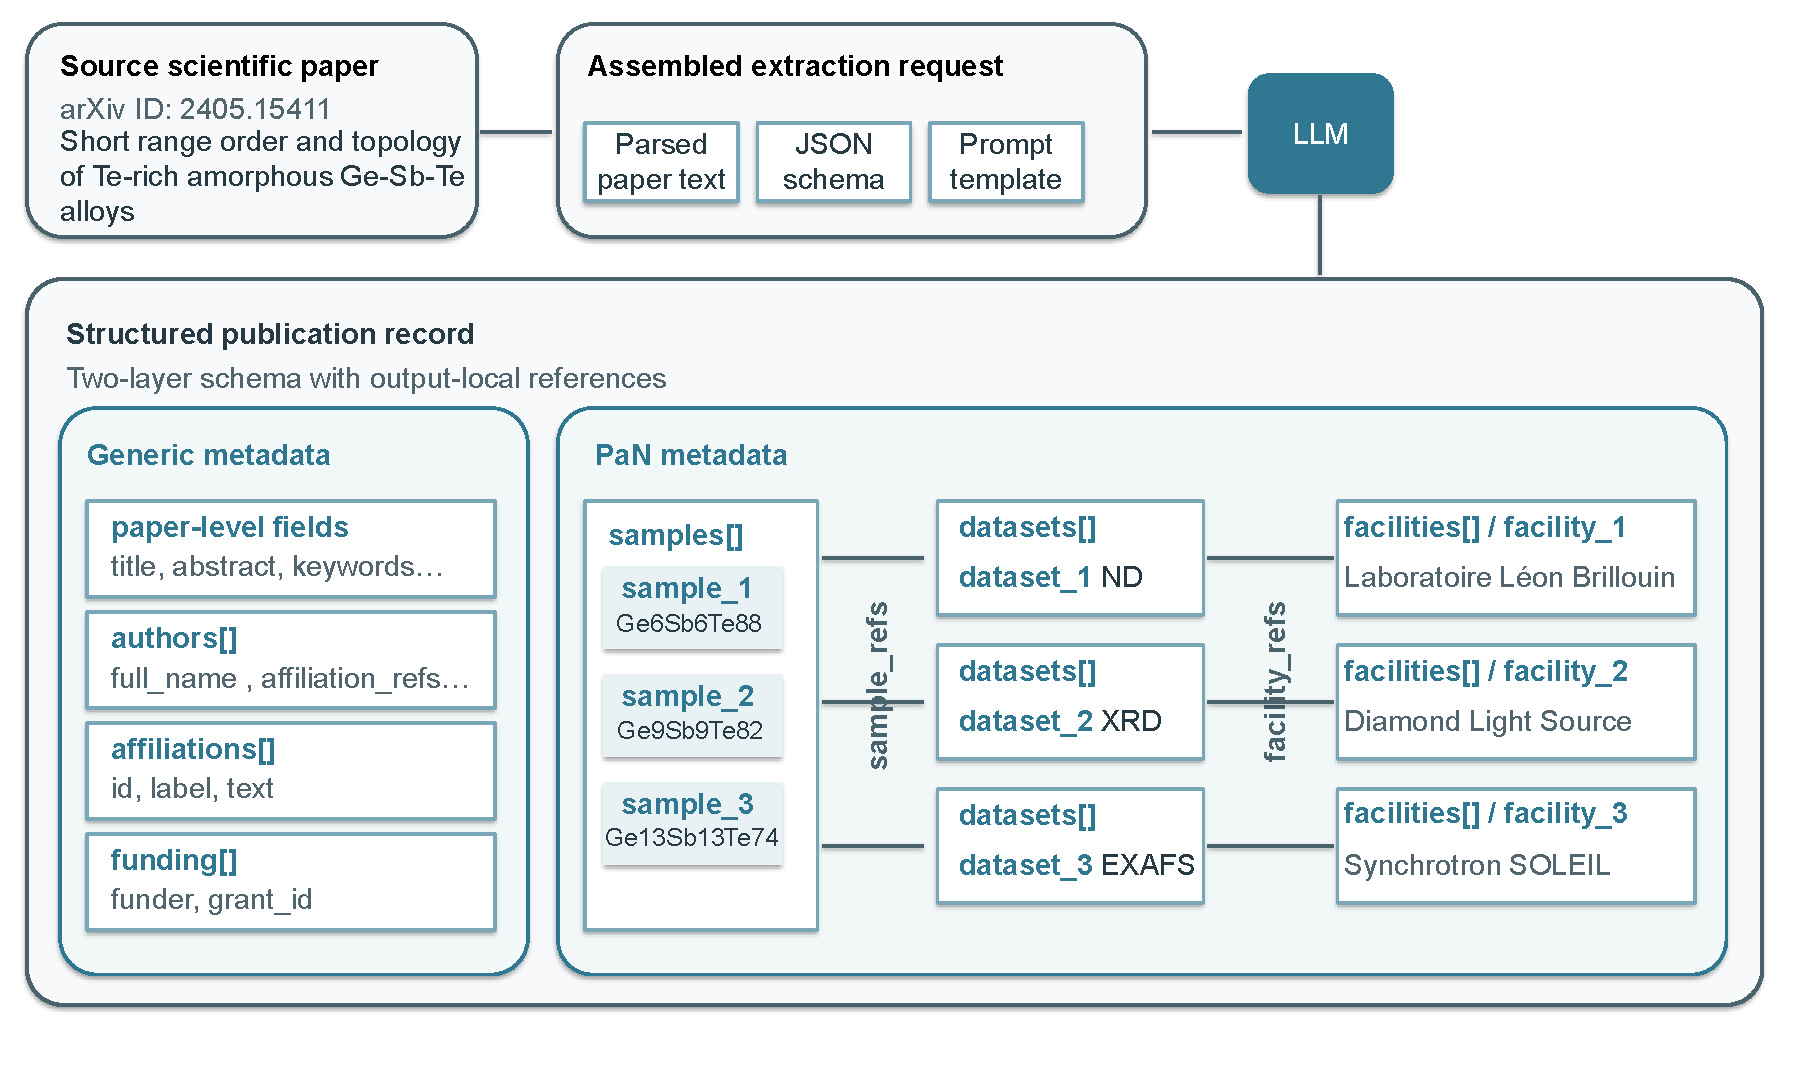
\includegraphics[width=0.95\textwidth]{figures/task_schema.pdf}
  \caption{Task and schema overview. Parsed content from a PaN scientific
  paper is combined with the prompt template and JSON schema to form the
  extraction request supplied to the LLM. The resulting structured publication
  record contains generic and PaN-specific metadata. The example is simplified
  from the reconciled gold record for arXiv:2405.15411, whose three datasets
  each reference the same three samples and one distinct facility. }
  \label{fig:task-schema}
\end{figure*}

\section{PaN Metadata Benchmark}
\label{sec:benchmark}

We formulate publication-derived PaN metadata extraction as the task of
recovering a structured metadata record from a scientific publication according
to a predefined schema. The target combines general publication metadata with
experimental information supported by the publication. We construct a benchmark
of 40 PaN publications for studying this task.

\begin{table}[t]
  \centering
  \small
  \begin{tabular}{@{}lr@{}}
    \toprule
    Item & Count \\
    \midrule
    \multicolumn{2}{@{}l}{\textbf{Corpus and annotation}} \\
    Papers & 40 \\
    Calibration papers & 10 \\
    Evaluation papers & 30 \\
    Working annotations & 90 \\
    \addlinespace
    \multicolumn{2}{@{}l}{\textbf{Repeated entities}} \\
    Affiliations & 179 \\
    Authors & 308 \\
    Funding items & 104 \\
    Facilities & 57 \\
    Samples & 127 \\
    Datasets & 118 \\
    \addlinespace
    \multicolumn{2}{@{}l}{\textbf{Paper-local reference edges}} \\
    Author--affiliation & 354 \\
    Dataset--sample & 321 \\
    Dataset--facility & 73 \\
    \bottomrule
  \end{tabular}
  \caption{Scale of the PaN metadata benchmark. Entity and
  reference counts are derived from the final gold records.}
  \label{tab:benchmark-statistics}
\end{table}


\subsection{Corpus Construction}
\label{sec:corpus}

The benchmark papers were selected from an initial pool of 116
publications retrieved through the arXiv API using technique-oriented search
queries. Selection was designed to cover a broad range of PaN experimental
techniques. Candidate papers were grouped to guide selection across 
small-angle scattering, diffraction, spectroscopy, imaging and tomography, 
reflectometry, and multi-technique studies, together with papers containing 
relatively sparse methodological detail. The resulting 40-paper corpus spans
varied experimental and reporting settings.

\subsection{Structured Metadata Schema}
\label{sec:task-schema}

We define the target metadata through two complementary schema layers. 
The generic schema is intended for reuse across scientific domains and 
captures publication identity and provenance, authors and affiliations, 
funding, and high-level document structure. The PaN schema represents 
experimental facilities, samples, and measurement datasets.

We select and adapt PaN fields from the DAPHNE4NFDI recommendations for 
experiment-time metadata capture \citep{lohstroh2025daphne}, retaining fields 
that can plausibly be supported by scientific publications. The PaN layer 
covers facility information, sample identity and characteristics, and 
dataset-level measurement information such as techniques, acquisition modes, 
and purposes. Together, the two layers define 15 paper-level fields and 
six entity collections, each allowing multiple structured entity records: 
affiliations, authors, funding items, facilities, samples, and datasets.

Each field specifies its semantics, value type, and applicable cardinality 
and structural constraints. Detailed field instructions define inclusion, 
normalization, and entity granularity.

Authors reference affiliations, and datasets reference samples and facilities 
through output-local identifiers such as \texttt{sample\_1} and \texttt{facility\_2}. 
These identifiers allow entities to be referenced by multiple records within an 
output. Their literal values are not globally stable scientific identifiers.

Figure~\ref{fig:task-schema} illustrates this structure using a simplified
excerpt from one reconciled gold record. The complete schema and detailed
field instructions are provided with the benchmark release.

\subsection{Annotation and Gold Construction}
\label{sec:annotation-gold}

Annotation was performed by three annotators. The 40-paper benchmark was 
divided into 10 calibration papers and a 30-paper evaluation set.

During calibration, all three annotators independently annotated the same
10 papers. Comparing these annotations exposed ambiguities in field inclusion,
normalization, entity granularity, and cross-entity references. These cases
were used to refine the schema, field instructions, and annotation protocol
before the evaluation papers were annotated.

The 30-paper evaluation set was divided into three 10-paper batches, with each
batch assigned to a different pair of annotators. Each annotator therefore
completed two batches, and every evaluation paper received two independent 
annotations. Together with the calibration annotations, this produced 90 working 
annotations.

Gold records were produced through reconciliation of the independent
annotations. For each evaluation batch, one annotator resolved disagreements
paper by paper against the source PDFs, and the second annotator reviewed the
resulting records. Reconciliation and review roles were rotated such that each
annotator served as reconciler for one batch and reviewer for another.
Calibration-paper disagreements were similarly resolved against the source
PDFs after protocol refinement. All reconciled records were expressed under
the final schema.

Table~\ref{tab:benchmark-statistics} summarizes the resulting benchmark. The 40
gold records contain 893 entity instances and 748 paper-local
references. In particular, 118 datasets are connected to samples through
321 dataset--sample references, reflecting that one dataset may involve
multiple samples and that one sample may be referenced by multiple datasets.
